% Tables are generated by experiments/build_manuscript_tables.py and
% experiments/summarize_split_sensitivity.py.
\subsection{Benchmark Datasets}

Nine public datasets were evaluated: five regression and four binary classification tasks (Table~\ref{tab:datasets}). The dataset inventory and all reported tables refer to the same experiments. Dataset sources, checksums, model predictors and split row positions are recorded with the results.

\begin{table}[htbp]
\centering
\small
\caption{Datasets and held-out samples. $p$ counts substantive predictors before one-hot encoding, excluding group identity and the intercept; $G$ counts groups. R: regression; C: classification. A and B give held-out rows; parentheses in B give held-out groups.}
\label{tab:datasets}
\begin{tabular}{lrrrrrr}
\toprule
Dataset & $n$ & $p$ & $G$ & Task & A & B ($G$) \\
\midrule
Sleepstudy & 180 & 1 & 18 & R & 36 & 40 (4) \\
ChickWeight & 578 & 2 & 50 & R & 143 & 144 (12) \\
MathAchieve & 7,185 & 4 & 160 & R & 1742 & 1792 (40) \\
Spruce & 1,027 & 1 & 79 & R & 237 & 247 (19) \\
Radon & 919 & 2 & 85 & R & 219 & 227 (21) \\
Contraception & 1,934 & 3 & 60 & C & 461 & 597 (15) \\
Toenail & 1,908 & 3 & 294 & C & 289 & 491 (73) \\
VerbAgg & 7,584 & 5 & 316 & C & 1896 & 1896 (79) \\
Train & 2,929 & 8 & 235 & C & 642 & 723 (58) \\
Exam & 4,059 & 6 & 65 & C & 989 & 935 (16) \\
\bottomrule
\end{tabular}
\end{table}

\FloatBarrier

\paragraph{Regression}
Sleepstudy predicts reaction time in milliseconds from Days, with subject-specific intercepts and slopes. ChickWeight predicts weight in grams from Time and categorical Diet, with chick intercepts. Machines predicts productivity score from categorical Machine, with worker intercepts. Oxboys predicts height in centimetres from standardized age, with subject intercepts and slopes; Occasion is not supplied to any method. Loblolly predicts tree height in feet from age, with seed-source intercepts.

\paragraph{Classification}
Aids2 predicts recorded final vital status from age, sex and transmission category, grouped by state. Observation times differ, so this is a descriptive binary task, not a fixed-horizon survival-risk analysis. Males predicts union membership from schooling, experience, ethnicity and industry, grouped by individual. VerbAgg predicts the dichotomized response from Anger, Gender, behavior type, situation and mode, grouped by respondent. Train predicts choice1 from the two alternatives' price, time, changes and comfort, grouped by respondent; the choice identifier is excluded. These outcomes and model predictors have no missing values in the downloaded versions.

\subsection{Experimental Setup}

\subsubsection{Two Prediction Regimes}

\textbf{Regime A: within-group observation holdout.} A random 25\% of observations, rounded down with a minimum of one, is held out separately within each group having at least two observations. At least one observation remains for every tested group. Singleton groups remain training-only. This evaluates prediction for known groups using their fitted information; it does not evaluate prospective forecasting beyond the observed time range.

\textbf{Regime B: out-of-group holdout.} A random 25\% of complete groups, rounded down with a minimum of one, is held out. No labeled support from these groups is available. TabMixNN uses zero random effects, and the classical mixed model uses its fixed part. For nonlinear models these are plug-in predictions at zero latent effects, not marginal integration over new-group variation. Kinship/GP extrapolation is not evaluated in this suite.

The primary tables use split seed 20261015, shared by all methods. A fixed sensitivity extension repeats both regimes with split seeds 20261016, 20261017, 20261018 and 20261019, keeping the model configurations and all three neural initialization seeds unchanged. These additional splits were specified after inspecting the primary analysis and are reported as an exploratory robustness analysis, not independent confirmatory validation. Test outcomes are used only for final evaluation. All categorical coding and numeric/target standardization are fitted on the training partition. Unseen categorical levels receive the training reference coding. The recorded split manifests permit exact reconstruction.

\subsubsection{Models and Training Budgets}

TabMixNN uses one hidden layer of width 32, embedding dimension 8, UN covariance and a Gaussian or binomial head. Each fit uses 2,000 full-batch Adam updates with learning rate 0.01, KL multiplier one, zero weight decay, no dropout, no centering and no extra structural penalties. Full batches retain source row order. The structural backbone options are disabled in the main comparison. Three initialization seeds (42, 123 and 456) are evaluated, without selecting the best seed. There is no test-driven hyperparameter search or early stopping.

The \textbf{fixed neural control} uses the same hidden architecture and budget with random terms removed. The \textbf{classical mixed baseline} uses the same fixed and random designs: Gaussian LMMs are fitted by ML using \texttt{lme4::lmer}; binomial GLMMs use \texttt{glmer} with the Laplace approximation \citep{bates2014fitting}. Known-group predictions include conditional fitted effects, whereas Regime B uses zero effects. Final optimizer convergence checks passed. On the primary split, the Aids2 and Train random-intercept fits were singular in both regimes. These boundary estimates are retained and reported; a fitted group-variance parameter need not be nonzero merely because a mixed model was specified.

\textbf{XGBoost} uses 200 trees, maximum depth 6 and learning rate 0.05 \citep{chen2016xgboost}. \textbf{Random Forest} uses 200 trees and minimum leaf size two. Both use seed 42. All methods receive the same substantive predictors; in Regime A, trees additionally receive training-fitted one-hot group indicators to make known-group information available. Trees receive no group indicators in Regime B. These are fixed comparator configurations, not exhaustively tuned methods.

\subsubsection{Metrics and Reproducibility}

Regression RMSE and MAE are reported in original outcome units after reversing training-target standardization; $R^2$ is also retained in the result files. Classification tables report AUROC and Brier score, with accuracy and log loss retained in those files. Lower Brier scores indicate smaller squared probability error; they alone do not establish calibration. Raw RMSE is not averaged across datasets with different units.

Neural entries in the primary tables are the mean and sample SD of metrics across three initialization seeds on the same test split. The sensitivity tables first average the metric over initialization seeds within each split, then report the mean and sample SD of these five split values. Repeated holdouts reuse observations and can repeat group partitions; these SDs describe sensitivity and are not standard errors. This SD does not estimate sampling uncertainty and is not a confidence interval. Classical and tree baselines use a single fit. No significance tests across datasets are claimed.

The executed environment used PyTorch 2.5.1, scikit-learn 1.9.1, XGBoost 3.2.0, R 4.4.1 and lme4 1.1-35.5. Scripts, versions, source checksums, per-seed metrics, baseline diagnostics and split manifests are provided in \texttt{experiments/}. The canonical suite is \texttt{run\_manuscript\_benchmarks.py}; tables are generated directly from its aggregate outputs. Source records and per-row predictions are cached locally and are not distributed with the manuscript.

\subsection{Results}

\subsubsection{Within-Group Regression}
TabMixNN has lower RMSE than the fixed neural control on all five known-group regression tasks. The comparison with other methods is task-dependent: XGBoost gives lower RMSE on Sleepstudy and Machines, whereas TabMixNN gives lower RMSE on ChickWeight, Oxboys and Loblolly. The large ChickWeight difference from the linear mixed model is consistent with the benefit of a nonlinear fitted response on this split; it does not by itself isolate a biological growth mechanism.

\begin{table}[htbp]
\centering
\small
\caption{Regression RMSE in original outcome units (lower is better). Regime A: observation holdout within known groups. Neural entries are mean $\pm$ sample SD over three initialization seeds on one fixed split; other methods use one fit. These SDs are not confidence intervals.}
\label{tab:regression_A}
\begin{tabular}{lrrrrr}
\toprule
Dataset (unit) & TabMixNN & Fixed NN & Mixed & XGBoost & RF \\
\midrule
Sleepstudy (ms) & $33.597 \pm 2.217$ & $48.007 \pm 0.269$ & 32.190 & 31.184 & 34.618 \\
ChickWeight (g) & $5.580 \pm 0.103$ & $40.278 \pm 0.389$ & 30.948 & 17.260 & 31.733 \\
Machines (score) & $1.021 \pm 0.122$ & $6.428 \pm 0.000$ & 3.431 & 0.656 & 2.528 \\
Oxboys (cm) & $0.847 \pm 0.009$ & $8.274 \pm 0.004$ & 0.926 & 1.864 & 4.430 \\
Loblolly (ft) & $0.812 \pm 0.147$ & $1.909 \pm 0.090$ & 2.582 & 1.989 & 1.882 \\
\bottomrule
\end{tabular}
\end{table}

\FloatBarrier

\subsubsection{Out-of-Group Regression}
Without observed outcomes from the test groups, the advantage is smaller. TabMixNN gives lower mean RMSE than XGBoost on three of five datasets (ChickWeight, Machines and Oxboys), but not on Sleepstudy or Loblolly. Machines has only one held-out worker. On Oxboys, TabMixNN's mean $R^2$ is approximately $-0.58$, and the other comparators also have negative $R^2$; a small RMSE advantage here should not be interpreted as useful generalization. The contrast between Tables~\ref{tab:regression_A} and~\ref{tab:regression_B} shows why the two prediction settings must be reported separately.

\begin{table}[htbp]
\centering
\small
\caption{Regression RMSE in original outcome units (lower is better). Regime B: entirely unseen groups, without labeled support. Neural entries are mean $\pm$ sample SD over three initialization seeds on one fixed split; other methods use one fit. These SDs are not confidence intervals.}
\label{tab:regression_B}
\begin{tabular}{lrrrrr}
\toprule
Dataset (unit) & TabMixNN & Fixed NN & Mixed & XGBoost & RF \\
\midrule
Sleepstudy (ms) & $29.985 \pm 1.696$ & $29.550 \pm 0.090$ & 29.446 & 29.644 & 29.407 \\
ChickWeight (g) & $41.224 \pm 0.598$ & $42.758 \pm 0.024$ & 41.078 & 42.751 & 42.702 \\
MathAchieve (score) & $6.235 \pm 0.014$ & $6.231 \pm 0.002$ & 6.107 & 6.407 & 6.750 \\
Spruce (logcm3) & $0.614 \pm 0.005$ & $0.611 \pm 0.002$ & 0.660 & 0.612 & 0.613 \\
Radon (log-pCi/L) & $0.735 \pm 0.002$ & $0.751 \pm 0.024$ & 0.711 & 0.862 & 0.814 \\
\bottomrule
\end{tabular}
\end{table}

\FloatBarrier

\subsubsection{Within-Group Classification}
Known-group classification also shows heterogeneous results. TabMixNN improves AUROC over the fixed neural control for Males, VerbAgg and Train, but not Aids2. The classical GLMM has the highest AUROC on Males, while TabMixNN has the highest mean AUROC on VerbAgg and Train. Probability-error rankings can differ from AUROC rankings, as the Brier scores show.

\begin{table}[htbp]
\centering
\small
\caption{Classification AUROC (higher is better) and Brier score (lower is better). Regime A: observation holdout within known groups. Neural entries are mean $\pm$ sample SD over three initialization seeds on one fixed split; other methods use one fit. These SDs are not confidence intervals.}
\label{tab:classification_A}
\begin{tabular}{llrrrrr}
\toprule
Dataset & Metric & TabMixNN & Fixed NN & Mixed & XGBoost & RF \\
\midrule
Contraception & AUC & $0.674 \pm 0.008$ & $0.669 \pm 0.001$ & 0.690 & 0.711 & 0.698 \\
Contraception & Brier & $0.228 \pm 0.006$ & $0.224 \pm 0.001$ & 0.216 & 0.211 & 0.216 \\
Toenail & AUC & $0.942 \pm 0.006$ & $0.687 \pm 0.010$ & 0.937 & 0.735 & 0.911 \\
Toenail & Brier & $0.057 \pm 0.004$ & $0.168 \pm 0.001$ & 0.065 & 0.154 & 0.126 \\
VerbAgg & AUC & $0.838 \pm 0.001$ & $0.696 \pm 0.004$ & 0.807 & 0.772 & 0.809 \\
VerbAgg & Brier & $0.165 \pm 0.002$ & $0.224 \pm 0.003$ & 0.179 & 0.197 & 0.183 \\
Train & AUC & $0.832 \pm 0.022$ & $0.739 \pm 0.025$ & 0.786 & 0.775 & 0.753 \\
Train & Brier & $0.179 \pm 0.014$ & $0.227 \pm 0.014$ & 0.192 & 0.193 & 0.211 \\
Exam & AUC & $0.796 \pm 0.004$ & $0.786 \pm 0.009$ & 0.816 & 0.807 & 0.773 \\
Exam & Brier & $0.187 \pm 0.002$ & $0.192 \pm 0.005$ & 0.175 & 0.180 & 0.199 \\
\bottomrule
\end{tabular}
\end{table}

\FloatBarrier

\subsubsection{Out-of-Group Classification}
The largest decrease in TabMixNN AUROC occurs for Males when individual-specific fitted information is unavailable. XGBoost performs better on that task. For VerbAgg, the mixed-model and TabMixNN AUROCs are close, while the fixed neural control has lower Brier error. Aids2 has only four grouping levels and holds out one state; all methods have AUROC near 0.5. These small-group results have limited support for broad extrapolation.

\begin{table}[htbp]
\centering
\small
\caption{Classification AUROC (higher is better) and Brier score (lower is better). Regime B: entirely unseen groups, without labeled support. Neural entries are mean $\pm$ sample SD over three initialization seeds on one fixed split; other methods use one fit. These SDs are not confidence intervals.}
\label{tab:classification_B}
\begin{tabular}{llrrrrr}
\toprule
Dataset & Metric & TabMixNN & Fixed NN & Mixed & XGBoost & RF \\
\midrule
Aids2 & AUC & $0.540 \pm 0.008$ & $0.529 \pm 0.010$ & 0.489 & 0.538 & 0.546 \\
Aids2 & Brier & $0.241 \pm 0.001$ & $0.242 \pm 0.002$ & 0.239 & 0.239 & 0.239 \\
Males & AUC & $0.620 \pm 0.020$ & $0.650 \pm 0.027$ & 0.651 & 0.723 & 0.674 \\
Males & Brier & $0.230 \pm 0.006$ & $0.211 \pm 0.008$ & 0.228 & 0.183 & 0.196 \\
VerbAgg & AUC & $0.697 \pm 0.007$ & $0.679 \pm 0.003$ & 0.700 & 0.668 & 0.663 \\
VerbAgg & Brier & $0.242 \pm 0.004$ & $0.230 \pm 0.001$ & 0.223 & 0.238 & 0.244 \\
Train & AUC & $0.737 \pm 0.003$ & $0.683 \pm 0.010$ & 0.723 & 0.702 & 0.668 \\
Train & Brier & $0.256 \pm 0.003$ & $0.267 \pm 0.004$ & 0.215 & 0.230 & 0.233 \\
\bottomrule
\end{tabular}
\end{table}

\FloatBarrier

\subsubsection{Linear Mixed-Model Check}
On Sleepstudy we additionally fit a scalar linear TabMixNN decoder using the same intercept/slope structure and split as the LMM. Regime-A RMSE is about 32.5 ms for linear VI and 32.2 ms for ML. This is a numerical check of predictions under a simple mean structure. It does not establish equality of variance estimates, posterior uncertainty or REML fitting, and it should not be extrapolated to the nonlinear benchmark model.

\begin{table}[htbp]
\centering
\small
\caption{Sleepstudy linear-model check: raw RMSE (ms). Linear VI uses a scalar identity decoder and unstructured intercept/slope covariance; lme4 fits the same linear mean and random-effects structure by ML. Near agreement of predictions does not imply identical covariance estimation or REML equivalence.}
\label{tab:linear_check}
\begin{tabular}{lrr}
\toprule
Regime & Linear VI & LMM (ML) \\
\midrule
A & $32.503 \pm 0.104$ & 32.190 \\
B & $29.292 \pm 0.141$ & 29.446 \\
\bottomrule
\end{tabular}
\end{table}

\FloatBarrier

\subsubsection{Ablation Studies}
Table~\ref{tab:ablation_comprehensive} compares seven configurations on the same Sleepstudy observation holdout. Removing random effects increases error relative to the intercept/slope model. Adding static or dynamic latent structure does not show a uniform improvement across seeds, and the comparison does not identify an optimal architecture. The three-seed variability and fixed update budget should be considered when interpreting small differences. No general recommendation about layer count or learning rate is inferred from this single dataset.

\begin{table}[htbp]
\centering
\small
\caption{Sleepstudy component comparisons on the same Regime-A split. RMSE is in milliseconds. Entries are mean $\pm$ sample SD over three seeds. Except for the scalar linear decoder, all variants use one hidden layer of width 32 and embedding dimension 8; all use the same 2,000-update budget. Structural variants use feature mixing without sparsity or contraction penalties. This is a component comparison, not a hyperparameter search.}
\label{tab:ablation_comprehensive}
\begin{tabular}{lrr}
\toprule
Configuration & RMSE $\downarrow$ & $R^2$ $\uparrow$ \\
\midrule
Intercept + slope & $33.597 \pm 2.217$ & $0.597 \pm 0.054$ \\
Intercept only & $33.900 \pm 1.646$ & $0.590 \pm 0.039$ \\
Fixed only & $48.007 \pm 0.269$ & $0.180 \pm 0.009$ \\
Linear decoder & $32.503 \pm 0.104$ & $0.624 \pm 0.002$ \\
Static & $32.312 \pm 2.473$ & $0.627 \pm 0.058$ \\
Dynamic & $31.940 \pm 0.444$ & $0.637 \pm 0.010$ \\
Gated static + dynamic & $32.013 \pm 0.965$ & $0.635 \pm 0.022$ \\
\bottomrule
\end{tabular}
\end{table}

\FloatBarrier

\subsubsection{Sensitivity to the Data Split}
\begin{table}[htbp]
\centering\small
\caption{Raw-unit RMSE over five fixed repeated holdouts. Each neural split value is the mean metric across three initialization seeds. Entries are mean $\pm$ sample SD across split values. Reused observations and repeated group partitions make these descriptive SDs, not standard errors or confidence intervals.}
\label{tab:split_regression}
\resizebox{\textwidth}{!}{%
\begin{tabular}{llrrrrr}
\toprule
Dataset & Regime & TabMixNN & Fixed NN & Mixed & XGBoost & RF \\
\midrule
Sleepstudy (ms) & A & $27.058 \pm 5.256$ & $47.695 \pm 3.950$ & $25.727 \pm 4.826$ & $26.666 \pm 3.003$ & $28.927 \pm 5.423$ \\
Sleepstudy (ms) & B & $40.823 \pm 9.597$ & $39.711 \pm 10.872$ & $38.571 \pm 10.993$ & $39.643 \pm 11.018$ & $39.545 \pm 11.074$ \\
ChickWeight (g) & A & $6.175 \pm 0.480$ & $36.383 \pm 3.018$ & $29.408 \pm 1.174$ & $16.237 \pm 0.622$ & $28.496 \pm 2.493$ \\
ChickWeight (g) & B & $38.728 \pm 4.357$ & $38.915 \pm 5.008$ & $39.998 \pm 5.617$ & $38.952 \pm 4.941$ & $38.946 \pm 4.833$ \\
Machines (score) & A & $1.143 \pm 0.213$ & $5.883 \pm 0.818$ & $3.133 \pm 0.321$ & $1.039 \pm 0.342$ & $2.321 \pm 0.401$ \\
Machines (score) & B & $4.450 \pm 1.254$ & $5.661 \pm 1.316$ & $5.660 \pm 1.316$ & $5.661 \pm 1.316$ & $5.727 \pm 1.305$ \\
Oxboys (cm) & A & $0.731 \pm 0.069$ & $8.377 \pm 0.312$ & $0.849 \pm 0.058$ & $1.699 \pm 0.122$ & $4.009 \pm 0.244$ \\
Oxboys (cm) & B & $9.402 \pm 1.470$ & $9.685 \pm 1.250$ & $9.674 \pm 1.261$ & $9.755 \pm 1.346$ & $9.682 \pm 1.367$ \\
Loblolly (ft) & A & $0.869 \pm 0.121$ & $2.045 \pm 0.193$ & $2.942 \pm 0.591$ & $1.754 \pm 0.324$ & $2.017 \pm 0.184$ \\
Loblolly (ft) & B & $1.524 \pm 0.341$ & $1.468 \pm 0.395$ & $2.657 \pm 0.226$ & $1.429 \pm 0.403$ & $1.427 \pm 0.394$ \\
\bottomrule
\end{tabular}}
\end{table}

\FloatBarrier
\begin{table}[htbp]
\centering\small
\caption{AUROC over five fixed repeated holdouts. Each neural split value is the mean metric across three initialization seeds. Entries are mean $\pm$ sample SD across split values. Reused observations and repeated group partitions make these descriptive SDs, not standard errors or confidence intervals.}
\label{tab:split_classification}
\resizebox{\textwidth}{!}{%
\begin{tabular}{llrrrrr}
\toprule
Dataset & Regime & TabMixNN & Fixed NN & Mixed & XGBoost & RF \\
\midrule
Aids2 & A & $0.528 \pm 0.022$ & $0.541 \pm 0.021$ & $0.540 \pm 0.020$ & $0.520 \pm 0.030$ & $0.527 \pm 0.026$ \\
Aids2 & B & $0.561 \pm 0.022$ & $0.542 \pm 0.011$ & $0.514 \pm 0.026$ & $0.537 \pm 0.028$ & $0.536 \pm 0.026$ \\
Males & A & $0.890 \pm 0.014$ & $0.712 \pm 0.019$ & $0.900 \pm 0.017$ & $0.801 \pm 0.019$ & $0.891 \pm 0.021$ \\
Males & B & $0.644 \pm 0.032$ & $0.637 \pm 0.022$ & $0.659 \pm 0.033$ & $0.682 \pm 0.029$ & $0.645 \pm 0.016$ \\
VerbAgg & A & $0.840 \pm 0.017$ & $0.703 \pm 0.020$ & $0.817 \pm 0.015$ & $0.779 \pm 0.021$ & $0.808 \pm 0.021$ \\
VerbAgg & B & $0.703 \pm 0.011$ & $0.693 \pm 0.018$ & $0.716 \pm 0.012$ & $0.683 \pm 0.017$ & $0.674 \pm 0.015$ \\
Train & A & $0.817 \pm 0.011$ & $0.723 \pm 0.017$ & $0.765 \pm 0.019$ & $0.759 \pm 0.016$ & $0.723 \pm 0.023$ \\
Train & B & $0.736 \pm 0.007$ & $0.701 \pm 0.015$ & $0.742 \pm 0.026$ & $0.704 \pm 0.017$ & $0.693 \pm 0.018$ \\
\bottomrule
\end{tabular}}
\end{table}

\FloatBarrier

The five split values are an exploratory robustness check with the same fixed
training budget. They are neither five independent studies nor a substitute
for external validation. The five seeds produce only two distinct held-out
group partitions for Machines and three for Aids2 in regime B; the other
dataset/regime combinations have five distinct test partitions. No favorable
split or initialization is selected for reporting.

Across splits, TabMixNN retains lower mean RMSE than the fixed neural control
on all five known-group regression tasks. Its mean RMSE is lowest among these
comparators on ChickWeight, Oxboys and Loblolly, whereas the classical mixed
model is lowest on Sleepstudy and XGBoost on Machines. For unseen groups,
TabMixNN has the lowest mean RMSE on ChickWeight, Machines and Oxboys, but
the classical mixed model is lowest on Sleepstudy and Random Forest on
Loblolly. The large split SDs and repeated small-group partitions limit what
these rankings establish.

For classification, TabMixNN has the highest mean AUROC on VerbAgg and Train
in regime A. The mixed model is highest on Males, and all methods are close
to chance on Aids2. In regime B, TabMixNN has the highest mean AUROC only
on Aids2, at 0.561; XGBoost is highest on Males and the mixed model on
VerbAgg and Train. These comparisons support task-specific predictive
benefits, not a uniform advantage for unseen groups.

\subsubsection{Probability Calibration Diagnostics}
Calibration is assessed on the primary held-out predictions, without modifying
them. A logistic model of observed outcome on predicted log-odds estimates an
intercept and slope jointly, with probabilities clipped to $[10^{-6},1-10^{-6}]$
only for that diagnostic transformation. The table averages coefficients over
three separate fitted seeds, rather than evaluating a probability ensemble.
Repeated observations are dependent, so independent-row standard errors are
not reported. Mean probability error and fixed-bin summaries are also retained
for all classification comparators in the reproducibility artifact. These
checks complement discrimination and squared probability error; they do not
establish transportable calibration.

\begin{table}[htbp]
\centering\small
\caption{Primary-split TabMixNN probability diagnostics, averaged across three fitted seeds. The intercept and slope jointly fit $\operatorname{logit}P(Y=1)=a+b\operatorname{logit}(\widehat p)$ on held-out rows. Their ideal values are 0 and 1. They are descriptive estimates, without independent-row uncertainty assumptions; no test-set recalibration is applied.}
\label{tab:calibration}
\resizebox{\textwidth}{!}{%
\begin{tabular}{llrrrrr}
\toprule
Dataset & Regime & Observed & Predicted & Difference & $a$ & $b$ \\
\midrule
Contraception & A & 0.403 & 0.387 & -0.017 & -0.113 & 0.501 \\
Contraception & B & 0.389 & 0.416 & 0.027 & -0.286 & 0.468 \\
Toenail & A & 0.235 & 0.199 & -0.037 & 0.584 & 0.674 \\
Toenail & B & 0.202 & 0.045 & -0.157 & -1.076 & 0.082 \\
VerbAgg & A & 0.454 & 0.482 & 0.028 & -0.183 & 0.731 \\
VerbAgg & B & 0.489 & 0.523 & 0.034 & -0.090 & 0.406 \\
Train & A & 0.542 & 0.506 & -0.036 & 0.225 & 0.488 \\
Train & B & 0.527 & 0.515 & -0.012 & 0.102 & 0.229 \\
Exam & A & 0.518 & 0.520 & 0.002 & 0.005 & 0.684 \\
Exam & B & 0.492 & 0.425 & -0.067 & 0.197 & 0.514 \\
\bottomrule
\end{tabular}}
\end{table}

\FloatBarrier

All eight TabMixNN calibration slopes in Table~\ref{tab:calibration} are below
one, ranging from 0.132 to 0.731, indicating that the fitted log-odds are too
extreme under this diagnostic on the primary split. A mean probability close
to the observed event fraction does not resolve this problem: Aids2 in regime
A has a mean error of only $-0.002$ but a slope of 0.228. On Males in regime
B, the observed event fraction is 0.280 and the mean predicted probability
is 0.128, an underprediction of 15.2 percentage points. These results limit
the use of the fitted probabilities as absolute risks, even where
discrimination is useful. They do not assess posterior predictive coverage.

\subsection{Interpretability Analysis}

Figures~\ref{fig:ablation_days_effects}--\ref{fig:ablation_breakdown} are descriptive plots from a separate fit to all 180 Sleepstudy observations (seed 42, 2,000 updates, the same nonlinear architecture). All training rows form the background. Values are transformed back to milliseconds. The fixed-design Days column is perturbed while random-slope values and group indices remain fixed, as described in Section~\ref{sec:interpretation}.

% Generated assets: experiments/create_feature_ablation_plots.py.
% Legacy asset filenames are retained; the quantities are feature ablations.
\begin{figure}[htbp]
\centering
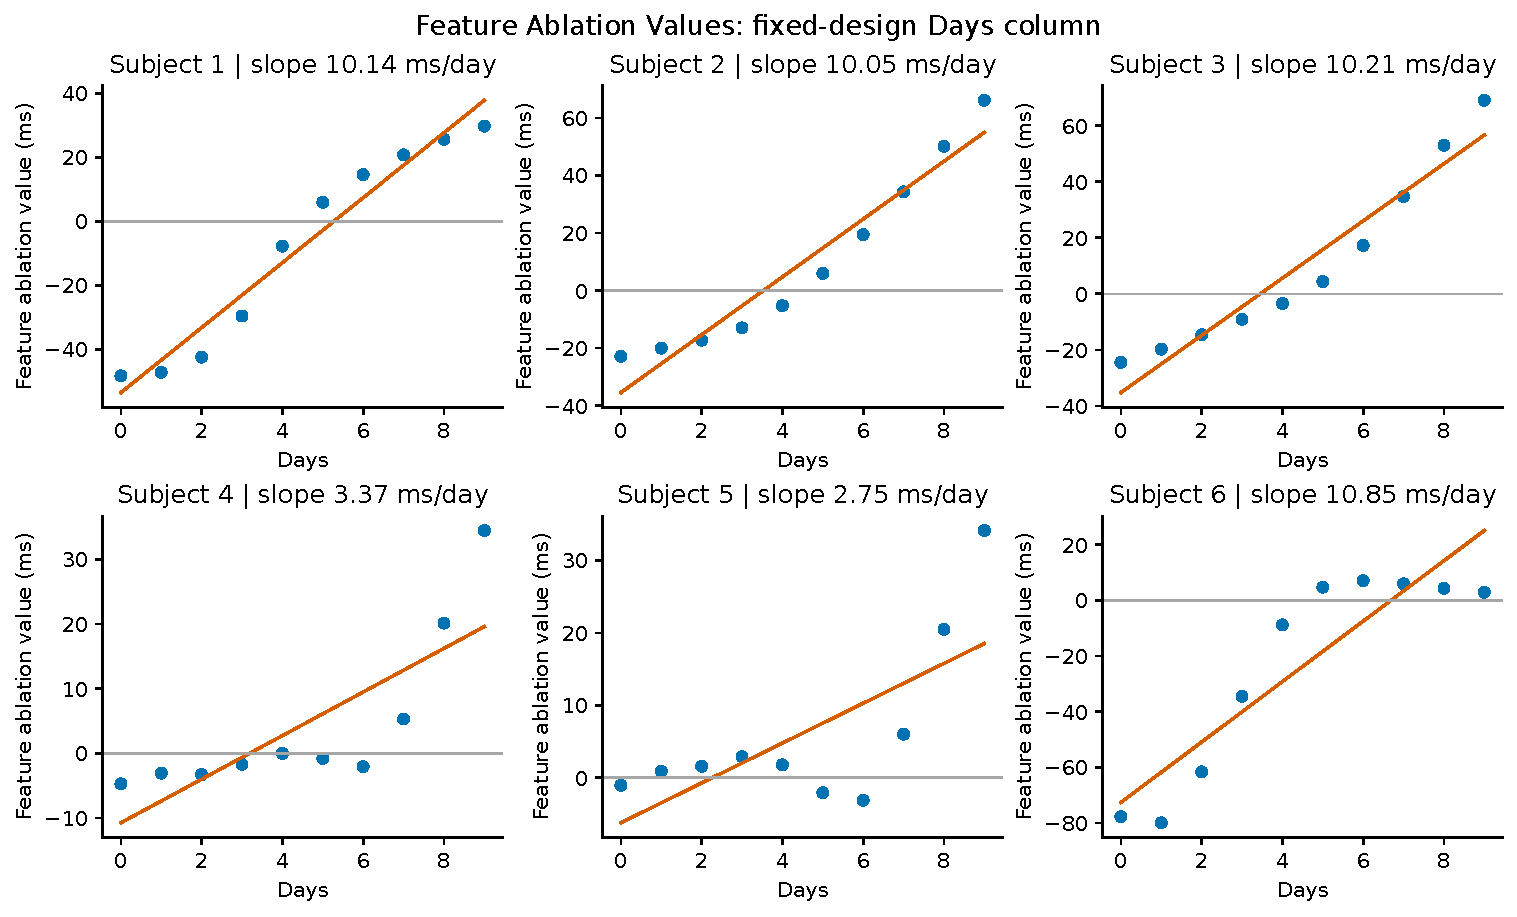
\includegraphics[width=\textwidth]{shap_days_effect_per_subject.pdf}
\caption{Fixed-design Days ablation values for six subjects, in milliseconds. Each point is the prediction minus its value after replacing the fixed-design Days column by the training-background mean, with the random-slope inputs and group indices held fixed. Lines are descriptive least-squares summaries, with slopes in ms/day. This is a full-data illustration, not held-out prediction assessment or recovery of subject-specific random coefficients. Subjects have anonymous source-order labels.}
\label{fig:ablation_days_effects}
\end{figure}

\begin{figure}[htbp]
\centering
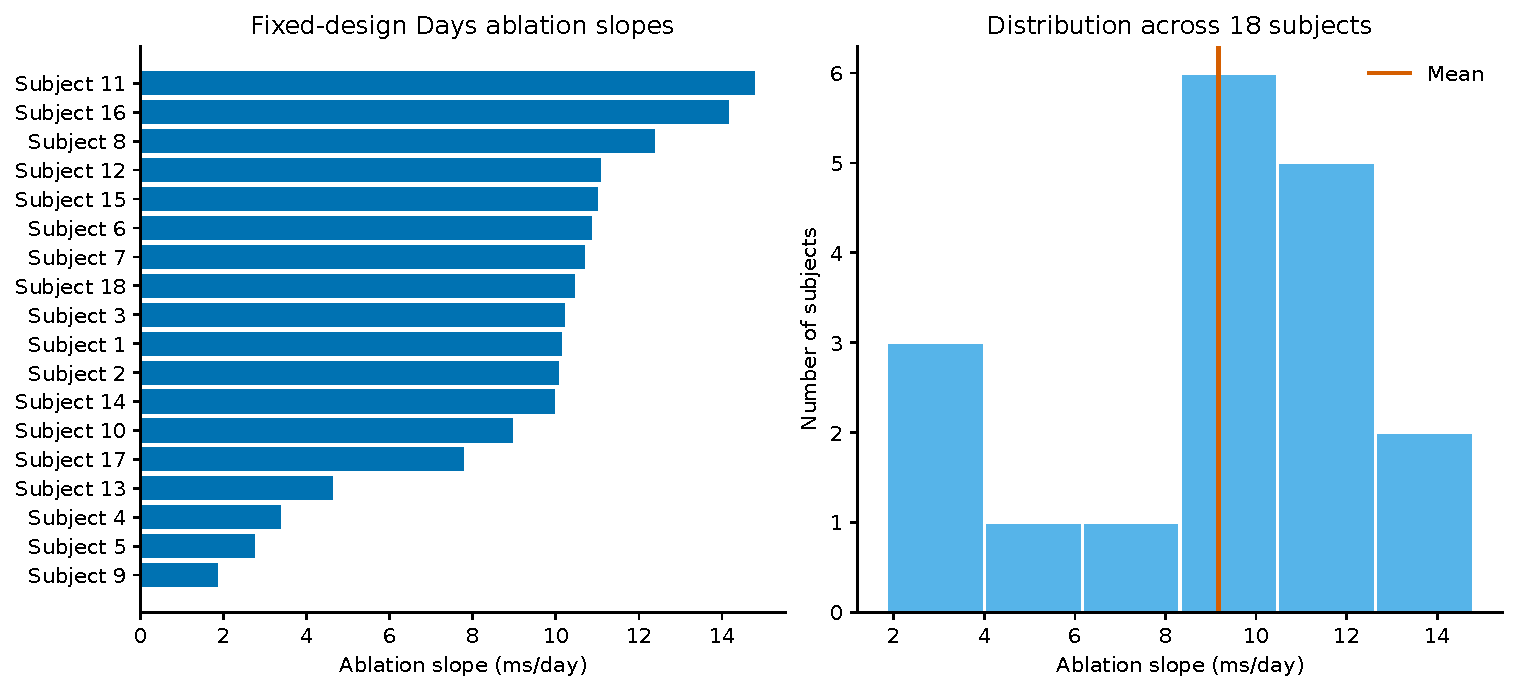
\includegraphics[width=\textwidth]{shap_subject_effect_comparison.pdf}
\caption{Ablation slopes from the fixed-design Days perturbation across all 18 subjects. Left: ordered descriptive line slopes in ms/day. Right: their distribution, with a line marking the mean. These summaries describe the fitted function under a specified perturbation; they do not estimate the random-slope variance component.}
\label{fig:ablation_subject_comparison}
\end{figure}

\begin{figure}[htbp]
\centering
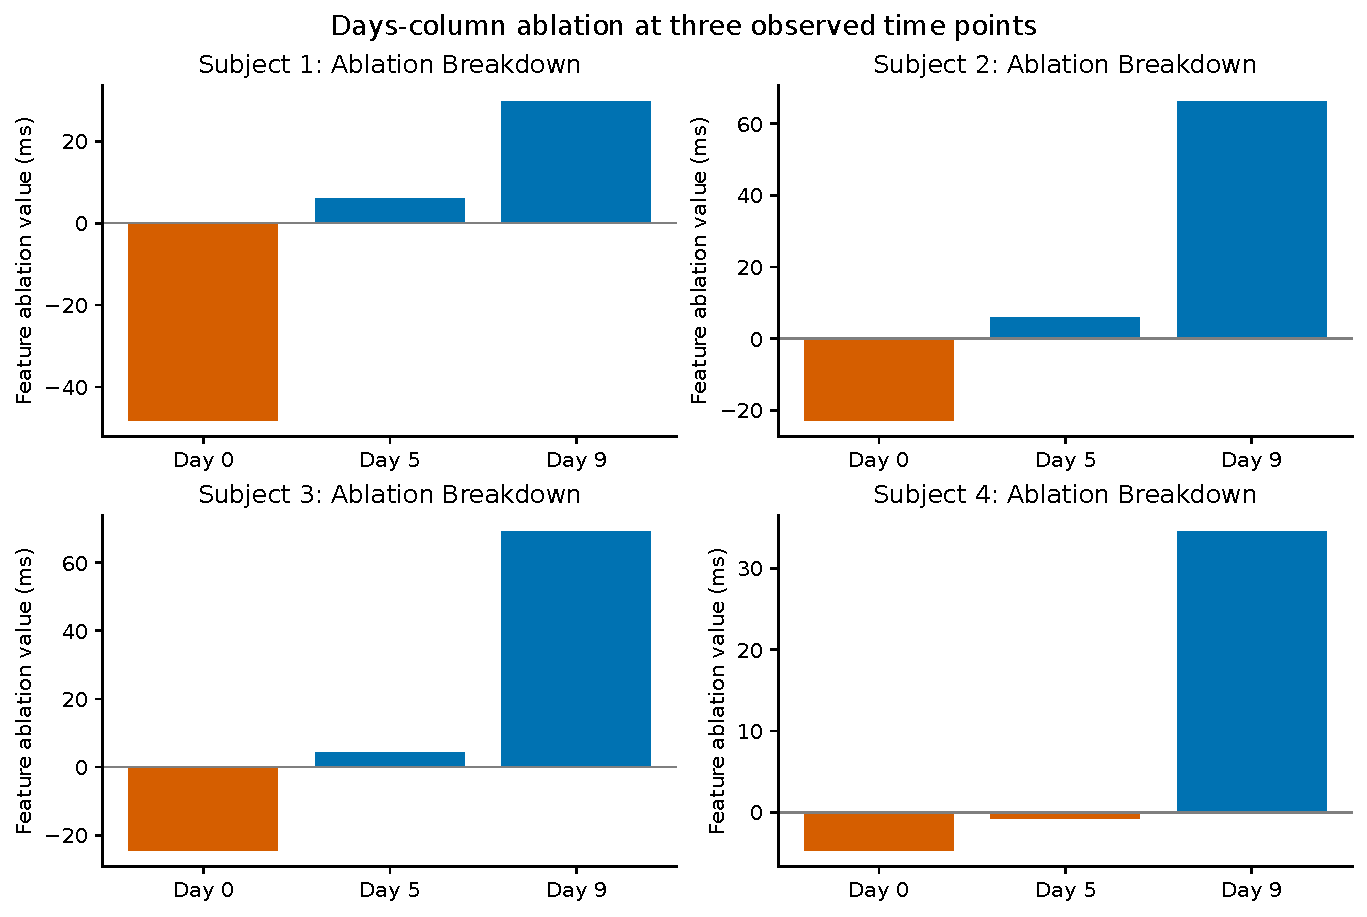
\includegraphics[width=0.95\textwidth]{shap_waterfall_subjects.pdf}
\caption{Ablation breakdown for four subjects at observed Days 0, 5 and 9. Bars show the single fixed-design Days-column prediction difference in milliseconds, using the same background and frozen random-slope inputs as Figure~\ref{fig:ablation_days_effects}. Bars describe separate observations and are not accumulated to reconstruct a prediction.}
\label{fig:ablation_breakdown}
\end{figure}

\FloatBarrier

The fitted lines in Figure~\ref{fig:ablation_days_effects} summarize the plotted perturbations; they are neither random-slope coefficients nor causal effects of sleep deprivation. Figure~\ref{fig:ablation_subject_comparison} summarizes their distribution. Figure~\ref{fig:ablation_breakdown} displays the same column perturbation at three observed days; its bars are not an additive decomposition of a prediction. The complete generator is \texttt{create\_feature\_ablation\_plots.py} in the experiments directory.

\subsection{Scope of the Empirical Evidence}

These experiments evaluate Gaussian regression, binomial classification and one component comparison. They do not evaluate survival prediction, multitask benefit, genomic prediction or the spatial manifold backbone. The repeated splits probe sensitivity to the held-out rows or groups, but limited model configurations leave tuning sensitivity unresolved. Specialized mixed-effects machine-learning baselines such as LMMNN and GPBoost are not evaluated. The package supports these additional interfaces, but no performance claim for them follows from the present results.
